\chapter{Preliminares}
\label{chap:basis}

En este capítulo se presentan los elementos fundamentales para el desarrollo de este trabajo. En la sección \ref{sec:definiciones-basicas} se presenta un conjunto de definiciones que serán utilizadas a lo largo del documento. Las otras secciones están dedicadas a las herramientas necesarias para automatizar la construcción de Generadores Multilenguajes en Common Lisp, que constituye el objetivo principal de este proyecto. Estas herramientas son: los Lenguajes de Dominio Específico (DSL), los Árboles de Sintaxis Abstracta (ASTs) y, por último, el lenguaje de programación Common Lisp, en el cual está implementada la herramienta propuesta en este trabajo.

\section{Definiciones básicas}
\label{sec:definiciones-basicas}

En la computación, existen diversos lenguajes para representar un problema de un área en particular. Esto obliga a los desarrolladores a escribir la misma solución en cada lenguaje donde desee emplearla. Un camino para simplificar el trabajo de los programadores en esta situación, sería implementar la solución en un Generador Multilenguaje.


\begin{definition}
  Un Generador Multilenguaje es una aplicación que define un DSL, y permite que los programas escritos en él puedan ser representados o exportados a varios lenguajes.
\end{definition}


Ejemplos de Generadores Multilenguajes son: Markdown \cite{markdown} y ORG-Mode \cite{emacs} que se especializan en exportar documentos a distintos formatos como HTML \cite{HTML}, LaTeX \cite{latex}, u ODT \cite{ODT}, a partir de un lenguaje de marcado que ellos definen; ADOL* es implementado en Common Lisp para representar Rutinas de Diferenciación Automática en varios lenguajes de programación \cite{Adol*}; Problemas de enrutamiento de vehículos (IVNS) \cite{cami}; Problemas de programación matemática (LAML) \cite{hoyos}.

\begin{definition}
  El dominio de un Generador Multilenguaje es el área de trabajo en que se especializa.
\end{definition}

El dominio de ADOL* es la Diferenciación Automática; el de Markdown, la edición de documentos; y el de LAML, los modelos de programación matemática \cite{hoyos}. 

\begin{definition}
	Un elemento del dominio representa una parte específica del área de trabajo.
\end{definition}

Algunos elementos en el dominio de Markdown son los textos, las listas de viñetas, y las referencias a documentos. En el dominio de (IVNS) se pueden encontrar los vehículos, los criterios de vecindad y las posibles rutas para los vehículos.

\begin{definition}
 Un lenguaje de salida es un lenguaje en el cual se desea representar los programas escritos en un Generador Multilenguaje.
\end{definition}

Entre los lenguajes de salida de Markdown se encuentran HTML, LaTeX, y ODT \cite{ODT}. En el caso de ADOL*, un lenguaje de salida, es cualquier lenguaje de programación que posea sobrecarga de operadores.   
 \begin{definition}
 Un Generador Multilenguaje es extensible si permite agregar nuevos lenguajes de salida.
 \end{definition}

 ADOL*, ORG-Mode y Markdown constituyen Generadores Multilenguajes extensibles. ADOL* permite agregar cualquier lenguaje de programación con sobrecarga en los operadores. ORG-Mode define una interfaz para implementar nuevos exportadores.


\section{Lenguajes de Dominio Específico}
Los ingenieros de software se encargan de encontrar herramientas para representar soluciones a problemas de las ciencias computacionales. Unas de las principales tendencias para la creación, modernización y mantenimiento de programas es el modelado de dominio especifico (\emph{DSM}) \cite{DSM}. Esta técnica propone crear abstracciones de los problemas para que los usuarios expresen fácilmente sus soluciones y ha sido utilizada en el desarrollo de lo que se conoce como Lenguajes de Dominio Específico (DSL). 

Un DSL es un lenguaje de programación destinado a aumentar la productividad de los usuarios al resolver un problema dentro de un contexto específico \cite{implementations_DSL}. Estos tienen la característica de ser típicamente más pequeños que los lenguajes de propósito general, pero al complementarse con otros ambientes de producción brindan un mejor nivel de abstracción sintáctico y semántico para la representación de un problema, permitiendo de esta forma ocultar las complejidades que aparecen en el proceso. Precisamente por ese motivo, y porque las herramientas actuales permiten crear nuevos lenguajes de programación con relativa facilidad, el uso de los DSLs es cada vez más frecuente \cite{dsl1}

En las siguientes secciones se presentan características de los DSLs relevantes para este trabajo: si son externos o internos y las etapas en su construcción.

\subsection{DSLs internos o externos}
Desde el punto de vista de la construcción del lenguaje, los DSLs se pueden clasificar en \textit{internos} o \textit{externos}. Los \textit{internos} forman parte de la sintaxis de un lenguaje de propósito general existente, usualmente en forma de librerías. Entre ellos se pueden mencionar Rails (construido en Ruby) \cite{ruby} y {ASP.NET Core} \cite{asp.netcore}, ambos orientados al desarrollo de aplicaciones web; el Sistema de Objetos de Common Lisp (CLOS) \cite{sonya} y Entity Framework \cite{entity}, un ORM (por sus siglas en inglés Object Relational Mapping) para .NET.
 
Los \textit{externos} se caracterizan por tener su propia sintaxis. Producto de que son construidos desde cero, estos tienen una sintaxis más especializada que los internos, pero requieren de la construcción de un compilador. Algunos ejemplos son {MATLAB}, para el trabajo con matrices y cálculos científicos \cite{matlab}; Graphviz, orientado al dibujo de grafos \cite{graph}, y R, cuyo propósito es brindar un lenguaje de programación orientado al trabajo estadístico \cite{R}.

\subsection{Construcción de un DSL}

En la literatura sobre Lenguajes de Dominio Específico se han identificado cinco etapas en la construcción de un DSL: \textit{Decisión}, \textit{Análisis}, \textit{Diseño}, \textit{Implementación} y \textit{Despliegue} \cite{dslEngineering} \cite{implementations_DSL} \cite{dsl1}.

En la etapa de \textit{Decisión} se investiga si es factible o no crear un DSL para el dominio seleccionado; posteriormente, en la etapa de \textit{Análisis} se investigan los elementos necesarios para modelar dicho dominio. Durante la etapa de \textit{Diseño}, se elige un lenguaje de programación en el cual implementar el DSL y se considera qué patrón de diseño utilizar \cite{dslEngineering}. Terminadas las etapas anteriores, corresponde la etapa de Implementación del DSL. Por último, se desarrolla la etapa de \textit{Despliegue}, que según Meyer \cite{meyer}, es la etapa más compleja durante la vida útil de un software.

En este trabajo, se implementó una herramienta para diseñar DSLs internos en Lisp, asumiendo que las etapas de \textit{Decisión}, \textit{Análisis} y \textit{Diseño} para la creación de un DSL están cumplidas correctamente. En la siguiente sección se presentan los {Árboles de Sintaxis Abstracta}, que resultan vitales para la etapa de Implementación de un DSL, y para la generación de código en los Generadores Multilenguajes.

\section{Árbol de Sintaxis Abstracta }
Un Árbol de Sintaxis Abstracta (AST, por sus siglas en inglés) es una estructura arbórea utilizada para representar segmentos de código escritos en programas computacionales.  Cada nodo del árbol contiene información recolectada durante el análisis lexicográfico y el sintáctico de un programa específico \cite{AST}. En la figura \ref{AST1} se muestra un AST correspondiente a la expresión $X= (Y+2) * (Z+3)$.  
Nótese que han sido eliminados los paréntesis y el punto y coma.

\begin{figure}
	\centering
	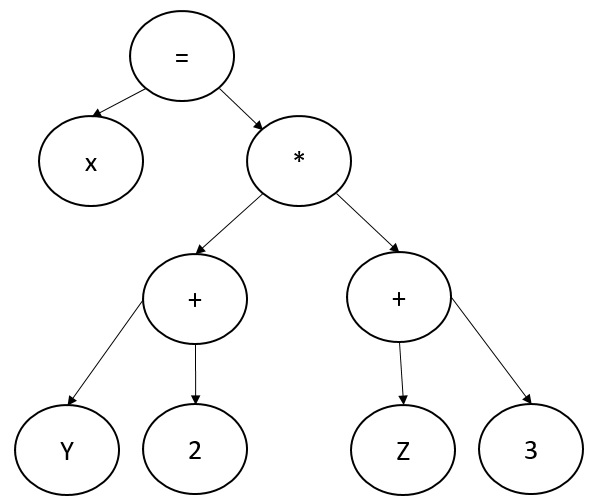
\includegraphics[width=0.6\textwidth]{AST1.png}
	\caption{AST correspondiente a la expresión: $X = (Y+2) * (Z+3);$}
	\label{AST1}
\end{figure}


Los nodos de un AST suelen ser instancias de clases diseñadas para representar cada operación del lenguaje, de forma que estos almacenen información necesaria de los elementos del dominio de un lenguaje de programación \cite{AST}. 

En {\gagm}, para generar el código fuente de un programa escrito en un DSL en cualquier lenguaje de programación, es necesario obtener el AST correspondiente. Para cumplir este objetivo, existen herramientas como ANTLR \cite{antlr} y YACC \cite{yacc}, aunque no siempre es necesario utilizarlas. Por ejemplo, en lenguajes como Ruby \cite{ruby} o Common Lisp \cite{clos-overview}, cuando el DSL que se está desarrollando es interno, no se requiere el uso de ninguna de las herramientas existentes para crear el AST de un programa, porque estos lenguajes brindan recursos propios, los cuales resultan más convenientes para la creación de este tipo de DSL. Además, como el objetivo de este trabajo es automatizar el proceso de Generadores Multilenguajes en Lisp, no es necesario realizar el análisis léxicográfico y sintáctico porque el intérprete de Lisp realiza esta tarea. La próxima sección está dedicada al lenguaje de programación Common Lisp.

\section{Common Lisp}

LISP es un lenguaje de propósito general creado en los años 50 por John McCarthy y fue desarrollado con el objetivo de crear un lenguaje que mostrara la información estructurada en listas, de ahí su nombre List-Processing \cite{ansi-common-lisp}.  Es el segundo lenguaje de alto nivel más antiguo que aún se utiliza en la actualidad, después de Fortran \cite{gentle-introduction-to-common-lisp}. La variedad de dialectos Lisp existentes en 1981 (Maclisp, Interlisp, zetalisp), provocó que en 1986 se creara el estándar llamado Common Lisp \cite{Land-of-Lisp}.

%Algunos de los escenarios en los cuales se emplea actualmente son La Inteligencia Artificial [paradig-lip] y el Procesamiento de Lenguaje Natural [natural proc lang in lisp].

Common Lisp es un lenguaje multiparadigma. En él, es posible crear programas orientados a objetos \cite{sonya}, completamente funcionales \cite{onlisp}, o cualquier combinación que se desee \cite{Land-of-Lisp}.  Posee un intérprete interactivo conocido por sus siglas REPL \cite{practical-common-lisp} y un Sistema de Objetos (CLOS) basado en herencia múltiple y funciones genéricas \cite{sonya}.

Las características que distinguen a Common Lisp del resto de los lenguajes de programación son su Sistema de Objetos y un Sistema de Macros que permite modificar el lenguaje para ajustarlo a las necesidades del usuario \cite{practical-common-lisp} \cite{sonya}. Estas son las razones fundamentales por la que se seleccionó Common Lisp para el desarrollo de este proyecto de tesis. El Sistema de Objetos simplifica la generación de código fuente en múltiples lenguajes de salida; y el Sistema de Macros, automatiza la construcción de lenguajes para los DSLs y la definición de los nodos de AST.

Para presentar las herramientas que facilitaron la implementación de \gagm, las siguientes secciones se dedican a la sintaxis de Common Lisp, a su Sistema de Objetos, y su Sistema de Macros.

\subsection{Sintaxis}

La sintaxis de Common Lisp es uniforme. Las funciones, los métodos, los macros y los operadores poseen todos la misma sintaxis.
\begin{verbatim}
                 (name arg1, arg2 … argN)
\end{verbatim}

% Ejemplos de esta sintaxis es el operador * y la función append. El operador * permite multiplicar varios números y la función append permite concatenar varias listas.
% 	\begin{verbatim}
% 	            (* 3 4 5)
% 	            (apppend ‘(“lista 1”) ‘(2 3) ‘(4 5))
% 	\end{verbatim}

Common Lisp no hace distinción entre las funciones propias del lenguaje y las funciones creadas por el usuario\cite{onlisp}. Esta característica permite crear y utilizar DSLs en Lisp con mucha facilidad \cite{Land-of-Lisp}. Por ejemplo, empleando funciones con nombres adecuados se puede construir un mini-lenguaje para elaborar páginas web en Lisp. Este lenguaje estará formado por las funciones \texttt{html}, \texttt{body} y \texttt{bold}, donde cada una devuelve la estructura correspondiente en HTML. Entonces una página sencilla se puede escribir como:
\begin{verbatim}
                 (html 
                   (body
                     "Un GM para" (bold "HTML")))
\end{verbatim}

\subsection{Funciones}

En Common Lisp, las funciones son Ciudadanas de primera clase \cite{onlisp}. En el contexto de los lenguajes de programación se dice que una entidad es Ciudadana de primera clase si puede ser utilizada en operaciones que comúnmente se realizan sobre los números o cadenas de texto: crear una nueva entidad en una rutina, almacenarla en variables o en estructuras de datos, incluirla en los parámetros de funciones o devolverla en llamados a funciones o macros \cite{onlisp}. Esta propiedad de las funciones permite automatizar las definiciones de los lenguajes para los DSLs.
  
Una función en Common Lisp acepta parámetros posicionales, opcionales, con nombre, o un número arbitrario de ellos. El conjunto de especificaciones en la definición de una función se conoce como Lambda List \cite{practical-common-lisp} (en otros lenguajes de programación se conoce como la signatura del método). Una selección apropiada de los nombres de las funciones y los parámetros de las mismas, en combinación con un uso adecuado de los elementos que brinda el lenguaje, permite crear código legible y fácilmente adaptable a cualquier dominio, como el que se muestra a continuación:
\begin{verbatim}
    (make-automation-recognizing (strings-over {0 1})
                                 (starting-with 1)
                                 (with-at-least 5 0)
                                 (ending-with 0))
\end{verbatim}

% A continuación, se define el Lambda Lisp de la función Suma:
% \begin{verbatim}
%                  (defun suma (&rest sumandos))
% \end{verbatim}

%La uniformidad en esta sintaxis facilita la creación de herramientas para desarrollar programas orientados a objetos en Common LISP.
En la siguiente sección, se presenta el Sistema de Objetos de Common Lisp, que resulta muy conveniente para representar los nodos de un AST y realizar la generación de código a múltiples lenguajes.

\subsection{Sistema de Objetos}

%En esta sección se presenta CLOS, el sistema de objeto de Common Lisp (En inglés, Common Lisp Object System).

El Sistema de Objetos de Common Lisp (CLOS, por sus siglas en inglés) es un conjunto de herramientas para desarrollar programas orientados a objetos \cite{sonya}. Está formado por clases que pueden tener herencia múltiple, instancias, funciones genéricas y métodos \cite{practical-common-lisp}. A diferencia de otros lenguajes de programación orientados a objetos, en CLOS los métodos no pertenecen a las clases, y no existe una sintaxis especial para referirse a las propiedades de sus instancias. A continuación, se describen los elementos de CLOS utilizados en este trabajo: clases, funciones genéricas y métodos.

\subsubsection{Clases en Common LISP}
\label{:sec clases en lisp}
El primer paso para escribir un programa en CLOS es implementar las clases, que definen la estructura y el comportamiento de objetos del mismo tipo \cite{sonya}\cite{clos-overview}.

Una clase en Common Lisp utiliza en su definición un conjunto de campos o propiedades (\textit{slots} en la terminología de CLOS) y opciones de clases. En dicho sistema de objetos se pueden construir clases a partir de otras clases (clases padres o super clases en la terminología de CLOS), de las cuales heredan sus \textit{slots} y comportamiento \cite{clos-overview}\cite{successful-lisp}.

Un ejemplo de la implementación de las clases \textit{operador binario} y \textit{suma} es:
\begin{verbatim}
(defclass binary-operator ()
    ((left-hand :accessor left-hand
          :documentation “The left value of the operator.”)
     (right-hand :accesor right-hand
          :documentation “The right value of the operator.”))
     (:documentation: “A binary node in the AST”))

(defclass sum-node (binary-operator)()
     (:documentation “A sum operator node in the AST”))
\end{verbatim}

La clase \texttt{binary-operator} representa un operador binario. Un operador binario tiene dos \textit{slots}, uno para el operador izquierdo y otro para el derecho. La clase \texttt{sum-node} hereda de la clase \texttt{binary-operator}.

Los \textit{slots} se definen para almacenar información del estado de una instancia en particular \cite{successful-lisp}. Para interactuar con ellos, se define un conjunto de opciones: \texttt{accessor} define el nombre de la función para acceder al valor del \textit{slot} correspondiente, \texttt{initarg} declara el nombre del parámetro, con el cual se inicializa el valor de un \textit{slot} en el momento de instanciar una clase, y el campo \texttt{documentation} almacena la documentación del \textit{slot} o la clase \cite{sonya}. Estas características de las clases serán automatizadas en la herramienta propuesta en este trabajo.

\label{Funciones constructoras}
Para crear una instancia de una clase en Lisp, se utiliza la función \texttt{make-instance}\cite{sonya}. Un patrón común para instanciar clases es utilizar funciones, métodos o macros ordinarios que reciben los valores con los que se desea instanciar una clase. El resultado de evaluar esas funciones, métodos o macros, son objetos creados a través de llamados a la función \texttt{make-instance}. En el resto de este documento estas funciones serán llamadas funciones constructoras.

Gracias a estas funciones constructoras, puede ser muy sencillo construir un AST en Lisp. Por ejemplo, la función constructora para la clase \texttt{sum-node} puede escribirse como:

\begin{verbatim}
         (defun + (left-hand right-hand)
                  (make-instance 'sum-node
                          :left-hand left-hand
                          :right-hand right-hand))
\end{verbatim}
Con esta definición, el resultado de evaluar \texttt{(+ 3 4)} es una instancia del nodo AST \texttt{sum-node}. Anidando llamados a las funciones constructuras se puede construir un AST de manera sencilla. En la figura \ref{AS2} de la página \pageref{AS2}, se puede observar el AST correspondiente al la expresión \texttt{(+ 3 (+ 4 5))}.

\begin{figure}
	\centering
	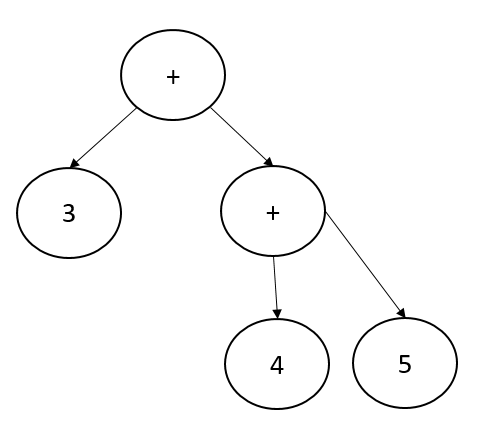
\includegraphics[width=0.4\textwidth]{AST2.png}
	\caption{AST correspondiente a la expresión: \texttt{(+ 3 (+ 4 5))}}
	\label{AS2}
\end{figure}

Una clase en Lisp puede heredar de varias clases \cite{sonya}. Esta característica resulta muy conveniente en el diseño de las jerarquías de nodos del AST y de los lenguajes de salida, lo que se puede observar en la sección \ref{sec:Jerarquía de lenguajes}.

El Sistema de Objetos de Common Lisp utiliza funciones genéricas para especificar las operaciones sobre las instancias de una misma clase \cite{practical-common-lisp}. 

\subsubsection{Funciones Genéricas y Métodos}
Una función genérica define solo una interfaz. Su comportamiento depende de la definición de su Lambda List, y su implementación se distribuye entre un conjunto de métodos\cite{cltl2}.
 
La función genérica que se presenta a continuación, se utiliza en ADOL* \cite{Adol*}, LAML \cite{hoyos} y IVNS \cite{cami} en la etapa de generación de código.
\begin{verbatim}
          (defgeneric generate-code node language stream)
\end{verbatim}

Esta función genérica es la clave para generar código hacia varios lenguajes. Recibe tres parámetros: \texttt{node}, \texttt{language} y \texttt{stream}; y sus métodos se especializan en generar el código correspondiente a cada nodo \texttt{node} del AST, en cada uno de los posibles lenguajes de salida, en un flujo de salida \texttt{stream}.

Por ejemplo, si se quiere generar el código del nodo \texttt{sum-node} en el lenguaje C\#, resulta necesario definir un método que implemente la función genérica \texttt{generate-code} y se especialice en el nodo \texttt{sum-node} y en el lenguaje C\#, como se muestra a continuación:
	
\begin{verbatim}
(defmethod generate-code ((node sum-node)(language csharp) stream)
    (format  stream “~a + ~a”
        (generate-code (left-hand node) language nil)
        (generate-code (right-hand node) language nil)))
\end{verbatim}
En CLOS, los métodos pueden ser extendidos por otros métodos llamados auxiliares\cite{let-over-lambda}. Estos se definen insertando una palabra clave \texttt{(:before, :after o :around)} después de su nombre y especificando el Lambda List del método que extienden \cite{sonya}. Dichos métodos, se utilizan para automatizar las características comunes en la sintaxis de los lenguajes de salida, lo que se ejemplificará en la sección \ref{lenguajesygcode}.

A pesar de ser una herramienta extremadamente poderosa \cite{sonya}, CLOS es solo un DSL interno en Common Lisp para el desarrollo orientados a objetos \cite{sonya}. Este sistema de objetos se pudo incluir en todos los dialectos de Lisp gracias a las funcionalidades del Sistema de Macros que se presentan a continuación.
\subsection{Sistema de Macros}
\label{macros}
Los macros en Lisp son estructuras sintácticas que permiten transformar fragmentos de código Lisp en otros fragmentos de código \cite{Land-of-Lisp}. Aunque los macros están presentes en varios lenguajes de programación como C++ y BASIC, los macros de Lisp trabajan de forma completamente diferente y a un nivel más sofisticado \cite{Land-of-Lisp}.

El Sistema de Macros de Common Lisp constituye una forma de extender la sintaxis del lenguaje \cite{onlisp}. Por ejemplo, en Common Lisp no está definida la sentencia \texttt{while} que posee el lenguaje de programación C\#. Sin embargo, en Common Lisp se puede definir un macro que implemente esta funcionalidad y permita escribir código como:
\begin{verbatim}
                    (while (< x 10)                                  
                       (setf x (+ x 1)))
\end{verbatim}

La instrucción \texttt{while} representa solo una básica sustitución de código, pero con esta idea se pueden crear DSLs para definir iteraciones complejas como el \texttt{Loop} de Common Lisp  \cite{onlisp}, un generador de HTML \cite{ansi-common-lisp} o un intérprete de PROLOG, este último en solo 145 líneas de código \cite{onlisp}.

Los macros se procesan en un tiempo diferente al que se evalúan las funciones o demás operaciones de un programa. Una función en Common Lisp se evalúa cuando se ejecuta un programa que la contenga (\textit{runtime}). Por otro lado, los macros se ejecutan cuando se lee y se compila el programa. Dicho momento se conoce como tiempo de expansión de macros (\textit{macro expansion time}, en inglés). Los parámetros de un macro no se evalúan en el momento en que estos son llamados, sino después de haber compilado el fragmento de código expandido por el macro \cite{onlisp}. La expansión de la llamada anterior al macro \texttt{while} sería:

\begin{verbatim}
                    (loop while (< x 10)
                        doing (setf x (+ x 1)))
\end{verbatim}

En este proyecto, los macros se utilizan para crear funcionalidades que permiten simplificar la creación de nodos del AST, definir automáticamente las funciones constructoras y encapsular fragmentos que se repiten en la generación de código. 

Con los elementos presentados en este capítulo es posible automatizar la creación de Generadores Multilenguajes en Common Lisp. En el siguiente capítulo se describe en detalle el proceso de creación de un Generador Multilenguaje, para posteriormente presentar cómo se puede automatizar cada uno de sus pasos.

%Hasta el momento, han sido presentados conceptos básicos sobre los Generadores Multilenguajes, DSLs, ASTs, así como las propiedades presentes en el Lenguaje de Common Lisp para diseñarlos e implementarlos.\\ 
%


%%% Local Variables:
%%% mode: latex
%%% TeX-master: "../Thesis"
%%% End:
